\clearpage
\section{Laser}

Our laser of choice, the LIDAR-Lite SEN-13167, is a SoC (System-on-a-Chip) solution for optical distance measurement applications. It has a 4.7 - 5.5 V nominal and 6 V potentially maximum DC operating range. The sensor has a theoretical limit of a 40m range and 100Hz rep rate. The laser emitters' accuracy is estimated to be +/- 2.5cm with an acquisition time of less then 20ms. These specifications allows us to get an accurate image of the environments specified in our test cases\cite{lidarsum}.

\begin{figure}[H]
	\centering
	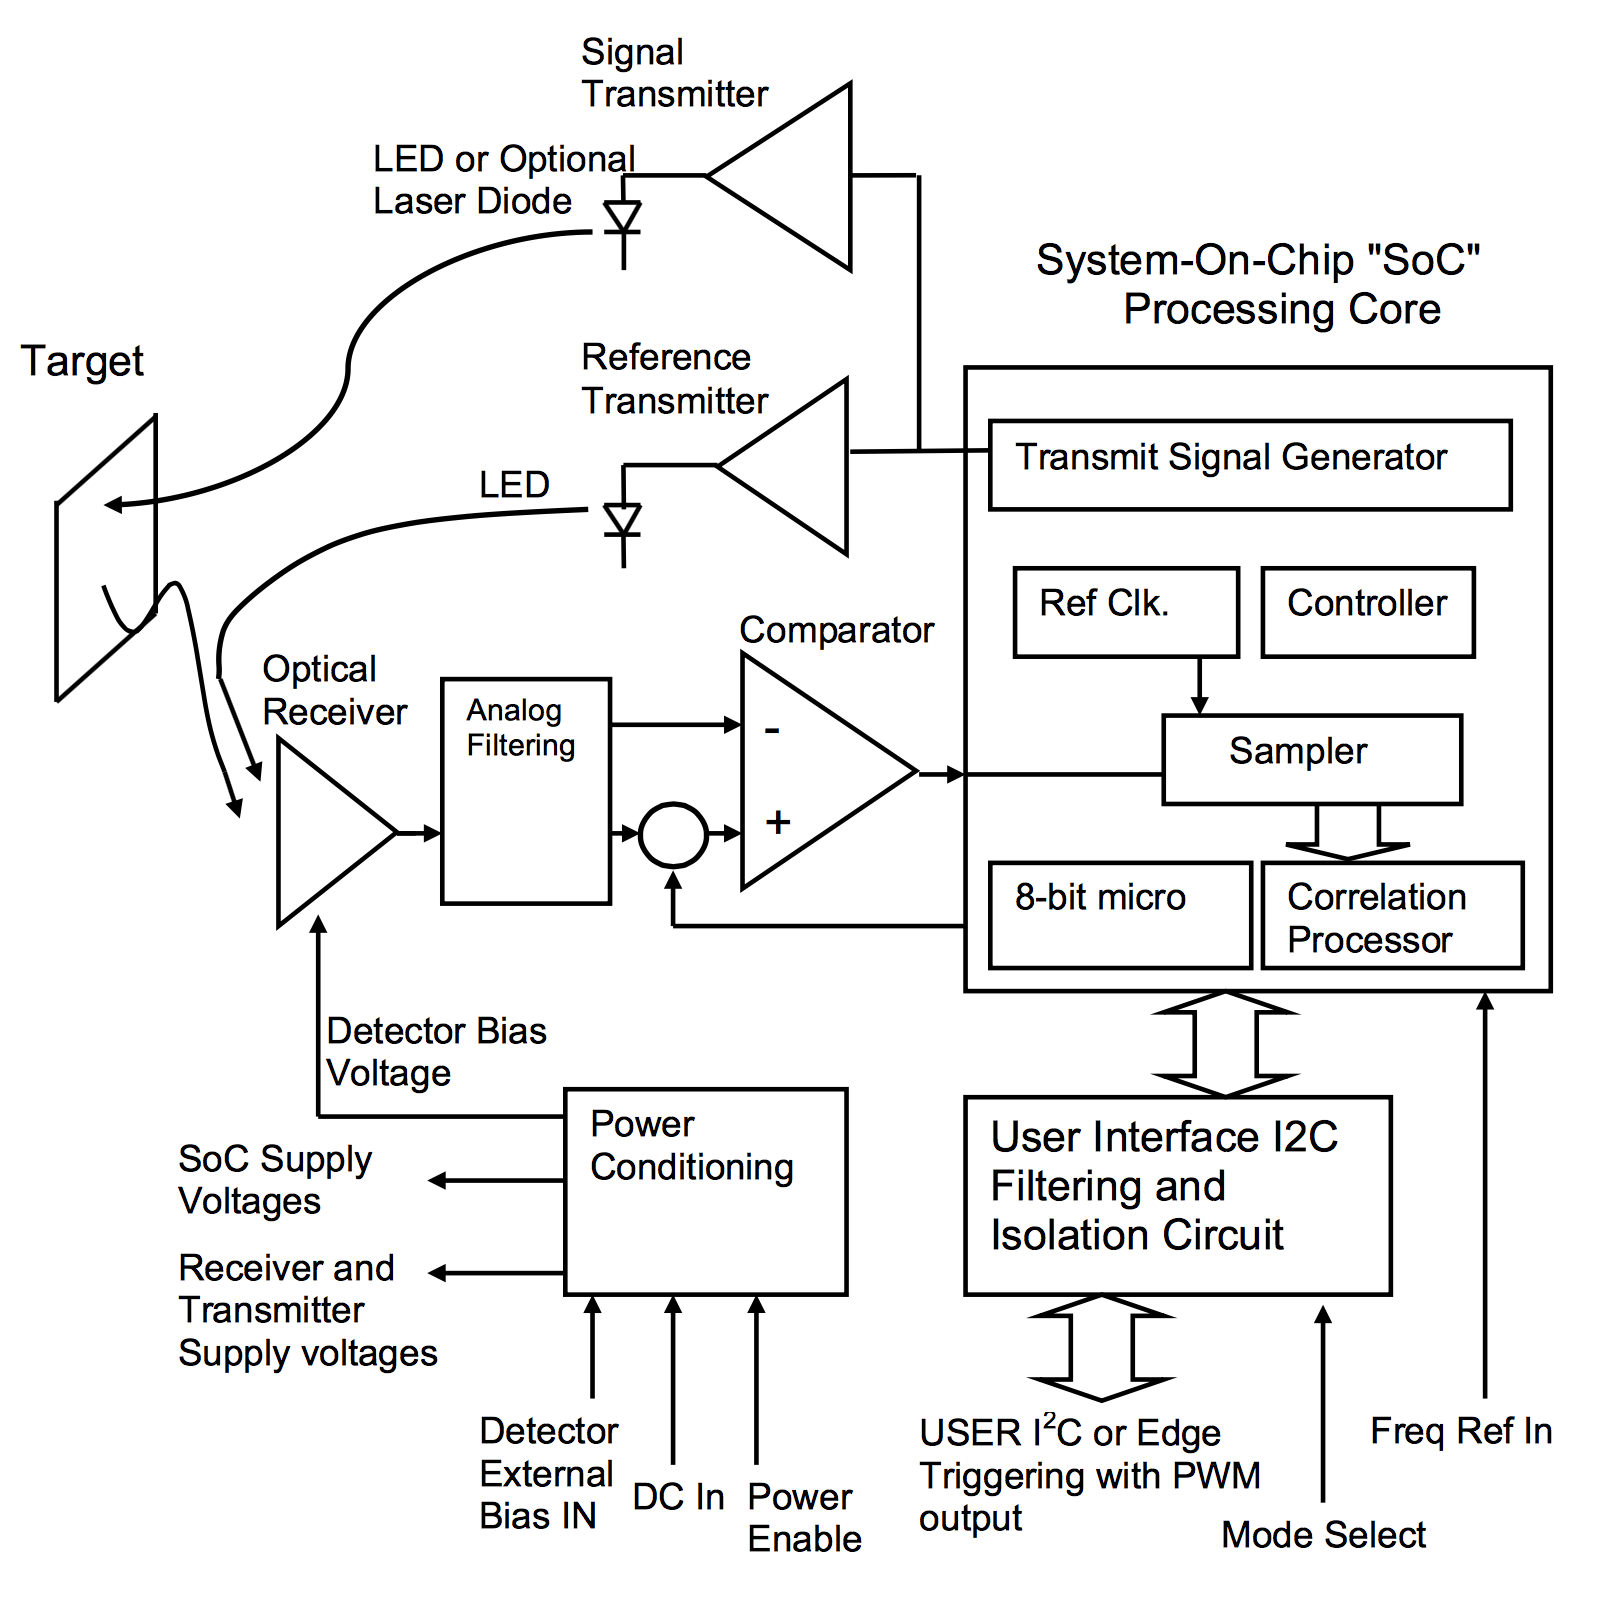
\includegraphics[scale=.4]{images/internallidar.png}
	\caption{An overview of the laser's internals\cite{lidarint}}
	\label{fig:internallidar}
\end{figure}

As previously discussed how the laser rangefinders work (Figure~\ref{fig:rangefinderIMG}), our laser has two 14mm optic lenses, one as a transmitter emitting a 905nm infrared (IR) pulse and a receiver, which is measuring the time it takes for the pulse to travel back and the angle at which it comes in.

At distances less than a meter, the pulse is about the size of the receiver's optic lens, and at distances longer than that, you can estimate it using the following equation: $\frac{d}{100} = psize$, where d = distance and psize = the pulse size at that specific distance, in the units they are measured in. The actual spread is $\sim 8$ Mil or $\sim\frac{1}{2}\degree$\cite{spreadofbeam}.

It is possible to receive multiple valid return signals from a single measurement if the pulse illuminates more than one surface along the beam path. The sensor has the capability to process two distinct reflections as long as they are separated by more than 3.5m and the reflection at the shorter distance does not saturate the correlation record masking the more distant object. 

Figure \ref{fig:tworeflections} shows an example of two reflections in the signal correlation record separated by approximately 3.5m.

\begin{figure}[H]
	\centering
	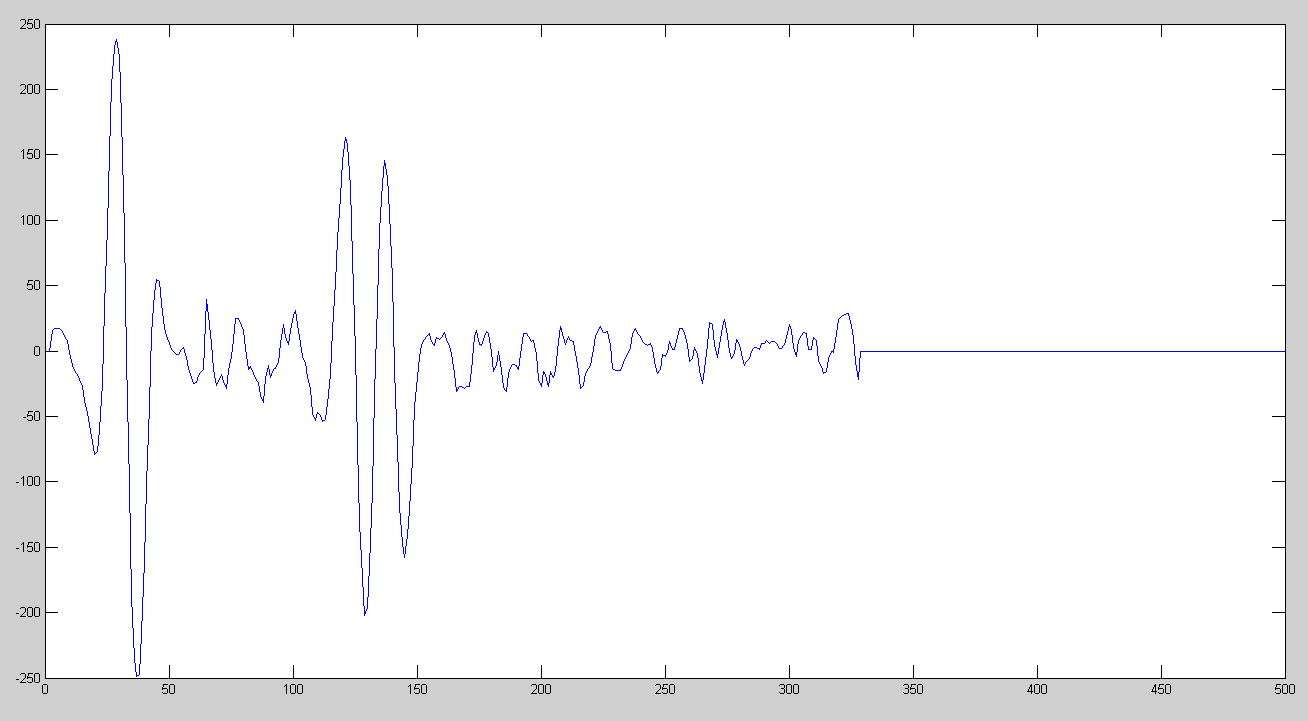
\includegraphics[scale=.3]{images/tworeflection.png}
	\caption{Measuring two valid return signals from one measurement~\cite{howtopulse}}
	\label{fig:tworeflections}
\end{figure}

The sensor detection criteria may be selected to pick the nearer signal, the more distant signal or the strongest signal strength. Currently, we do not handle multiple reflection in our code.

A reference signal is sent from the transmitter to the receiver, prior to the first distance measurement with a received pulse reflected from the target. The time delay between these two stored signals is estimated through a signal processing approach known as \textit{correlation}, which effectively provides a signature match between these two closely related signals. This accurately calculates the time delay, and is translated into distance based on the known speed-of-light, which is $\sim3.3ns\textbackslash m$\cite{howtopulse}.

By default, the sensor runs at about 50Hz, but could vary given the signal strength and distance. To optimize the rep rate, it is possible to decrease the max-acquisition count (on register 0x02). By default, register 0x02 is 0x80 (value 128 in decimal), if you decrease this, the maximum number of acquisitions the sensor can take and use to get a reading, will decrease, too\cite{reprate}.

\pagebreak

The assembling of the laser happened as shown on figure \ref{fig:wiringlidarpi}.

\begin{figure}[H]
	\centering
	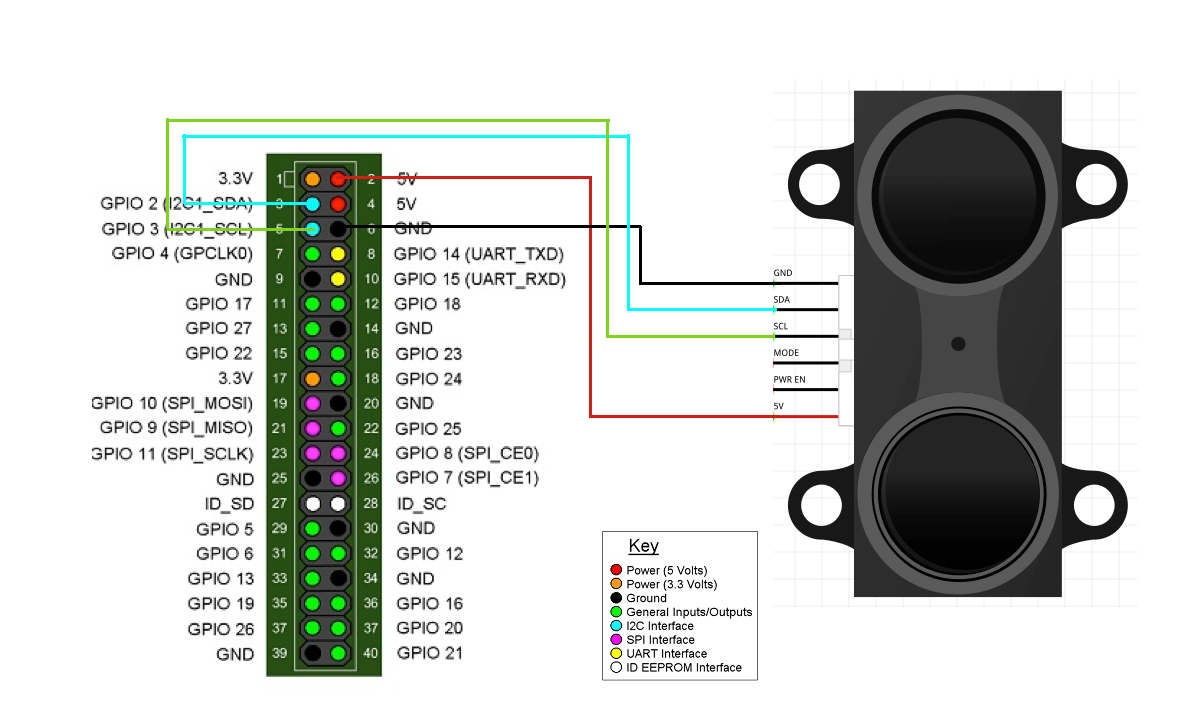
\includegraphics[scale=.35]{images/laderraspberryconnection.png}
	\caption{The pinout and wiring of the LIDAR-Lite laser and Raspberry Pi}
	\label{fig:wiringlidarpi}
\end{figure}

\begin{table}[H]
	\centering
	\begin{tabular}{|l|l|l|}
		\hline
		\textbf{Raspberry pin} & \textbf{Description} & \textbf{LIDAR pin} \\ \hline
		2 & 5V & Red \\ \hline
		5 & GND & Black \\ \hline
		4 & SCL & Green \\ \hline
		3 & SDA & Blue \\ \hline
	\end{tabular}
	\caption{The pins of the microcontroller mapped to the laser pins}
\end{table}

The laser can be interfaced through $I^2C$ (Inter-Integrated Circuit) or PWM (Pulsed Width Modulation)~\cite{lidarsum}. The default $I^2C$ address for the laser is 0x62, which we could validate by running the following command:
\lstset{language=sh}
\begin{lstlisting}
	>> $ sudo i2cdetect -y 1
	>> $
		  0  1  2  3  4  5  6  7  8  9  a  b  c  d  e  f
		  00:          -- -- -- -- -- -- -- -- -- -- -- -- --
		  10: -- -- -- -- -- -- -- -- -- -- -- -- -- -- -- --
		  20: -- -- -- -- -- -- -- -- -- -- -- -- -- -- -- --
		  30: -- -- -- -- -- -- -- -- -- -- -- -- -- -- -- --
		  40: -- -- -- -- -- -- -- -- -- -- -- -- -- -- -- --
		  50: -- -- -- -- -- -- -- -- -- -- -- -- -- -- -- --
		  60: -- -- 62 -- -- -- -- -- -- -- -- -- -- -- -- --
		  70: -- -- -- -- -- -- -- -- 
\end{lstlisting}

As the output shows, the address is available and the $I^2C$ connection is usable. The -y 1 relates to the revision B of the Raspberry Pi board.

We started using a library called lidarLite, which provides a simple C interface to the LIDAR-Lite laser on the Raspberry Pi. It is using the WiringPi access library written in C for the BCM2835 SoC, used on the Raspberry Pi. It is usable with C and C++ or many other languages with suitable wrappers. It was designed very familiarly to Arduino's wiring library~\cite{wiringPi-similarities}.

With the lidarLite library\cite{lidarlib}, we managed to read data using the $I^2C$ protocol. To do this, we had to enable the kernel support for $I^2C$ on the Raspberry Pi~\cite{i2csetup}.

A small program was been written in order to test the output of the laser sensor, to read out the distance value of the next closest point in centimeters. 

\lstinputlisting[firstline=20, lastline=36, title=sample output from our laser test code, language=C++]{../code/sampleOutput.txt}

This output is generated by the function called \textit{lidar\_read(int fd)} from the lidarLite library. This code simply calculates by low and high value from the sensor returns the distance measurement in centimeters, in form of an integer value.

\clearpage

\lstinputlisting[firstline=47, lastline=64, title=lidarLite.c, language=C]{../code/lidarlite_scan/src/lidarLite.c}

We tried to incorporate this measurement code with a stepper-motor, so that it would return the distances around a circle. The first version had the stepper-motor spinning the laser around at a constant speed, which was driven by an Arduino board (Code reference ~\ref{code:arduinocode}), while the laser made measurements that was driven by the Pi.

In order to determine how long it takes for the lidarLite \textit{lidar\_read(int fd)} function to execute, some testing was made.

\lstinputlisting[firstline=1, lastline=8, title=laserTiming.cpp, language=C++]{../code/asd.cpp}

This code was run with the settings of 1000 and 2000, and each version was ran 3 times. The time was measured using the UNIX \textit{time} utility.

Measurements of how long it takes to run \textit{lidar\_read(int fd)}:

\begin{table}[H]
	\centering
	\begin{tabular}{|l|l|l|l|l|} \hline
            Number of Calls & Measurements & & & Average \\ \hline
            1000 & 24.372s & 24.476s & 24.490s & 24.446s \\ \hline
            2000 & 48.400s & 48.111s & 48.172s & 48.228s \\ \hline
	\end{tabular}
	\caption{Data from testing}
\end{table}

According to this data, we can isolate the time it takes to execute the \textit{lidar\_read(int fd)} function from everything else:

$t_{total} = n*t_{lidar} + t_{rest}$ \\

$24.446s = 1000*t_{lidar} + t_{rest}$ \\
$48.228s = 2000*t_{lidar} + t_{rest}$ \\

Subtract the two equations:

$23.782s = 1000*t_{lidar}$ \\
$t_{lidar} = 0.023782s \approx 0.024s$ \\

This proved ineffective, since the rotation and measurements were independent from each other. If the time for one measurement is not precise enough the measurements to be skewed over time.

We then attempted to control the stepper-motor with the Raspberry Pi, added to the same code as we were running the laser with. However, the wiringPi library required root privileges, and ROS was not designed to be run under root privileges. The solution was to use a system call library to call an external file, which then would drive the stepper-motor. This makes the stepping and measuring synchronous, but making system call is very expensive in terms of computational resources, meaning that the code is significantly slower than the top speed that the laser is capable of.

The full code written for the laser sensor can be found in Appendix \ref{code:laser-full}. The sequence diagram shown in figure \ref{fig:lasermodule} gives us an overview of the calls happening in the code.

\begin{figure}[H]
	\centering
	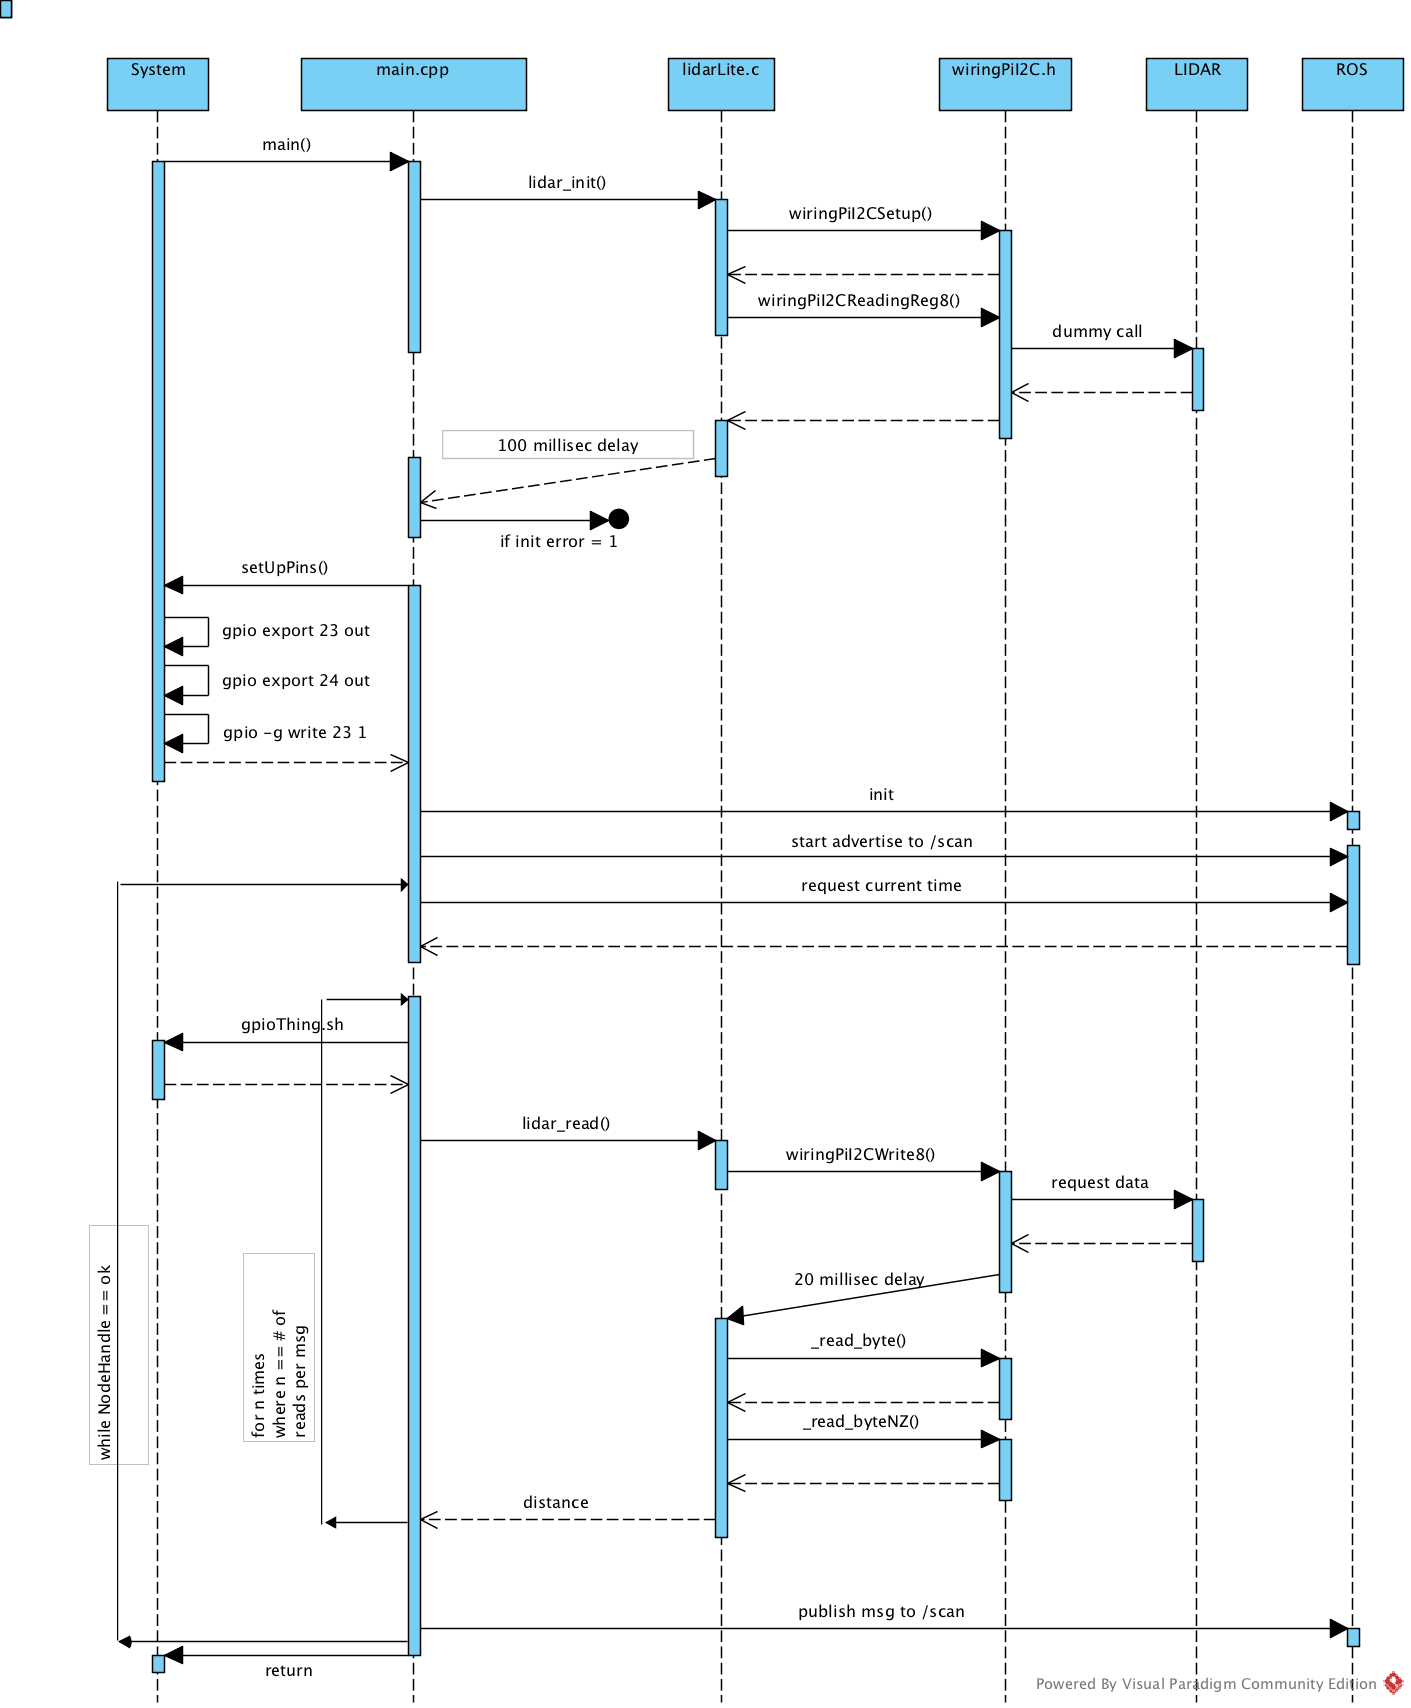
\includegraphics[scale=.6]{images/laser-module.png}
	\caption{Sequence diagram of the main function call in main.cpp}
	\label{fig:lasermodule}
\end{figure}

The first step is to initialize the the LIDAR-Lite laser sensor, by giving a dummy "wake-up" call to it via the wiringPi library, using the $I^2C$ protocol. There is a 100 millisec delay, which is necessary for the device to wake up and for the reading of registry to be completed. If the initialization fails, the program terminates by printing out a message to the terminal.

Thereafter, we call the \textit{setUpPins()} function which makes the system call 3 separate calls using the GPIO utility, setting up the GPIO on the Raspberry Pi to be able to communicate with the stepper motor.

The initialization of ROS happens afterwards, by calling the \textit{init} function with arguments and the name of our module. The module name is used as the node name in ROS. In the next line, ROS also starts to advertise messages to the \textit{/scan} topic, where all the scan results are being published to.

The rest of the code consists of two loops, one \textit{while} loop and one \textit{for} loop. The \textit{while} loop continues until the node returns anything other than an \textit{OK} status code. In here, a new LaserScan variable is being created where we ask ROS for the current time, set some hardcoded values and populate an array with the readings. The \textit{for} loop is then used to get 200 readings from the LIDAR-Lite laser using the \textit{lidar\_read(fs)} function and also rotating the stepper motor before each of the calculation using the \textit{step(num\_step)} function. The \textit{step(num\_step)} function is calling a shell script that is doing calls to the GPIO interface, making the stepper motor to take 8 micro-steps, or in other terms, one full step. Before the end of the \textit{while} loop, the message is being published to \textit{/scan}.

\lstinputlisting[firstline=1, lastline=16, title=gpioStuff.sh, language=sh]{../code/gpioThing.sh}

The only purpose of the code above, is to be called from the main file. The gpio utility is capable of interfacing with the GPIO pins on the Pi without root privileges. The change from low to high causes a micro-step, and 8 micro-steps makes one full step.

\clearpage
\subsection{Laser Safety Analysis}

In the following section we analyse and review the classification of the laser product of choice, the LIDAR-Lite rangefinder laser. 

This product emits laser radiation and it is classified as a \textit{Class 1 laser product} during all procedures of operation. This means that the laser is safe to look at with the unaided eye, however, it is very advisable to avoid looking into the beam and power the module off when not in use\cite{laserclass}.

The operation of LIDAR-Lite, without proper housing and optics, or modification of the housing or optics that exposes the laser source may result in direct exposure to laser radiation and the risk of permanent eye damage. Removal or modification of the diffuser in front of the laser optic may result in the risk of permanent eye damage and the declassification of the laser as a \textit{Class 1 laser product}. The product is also RoHS compliant\cite{laserrohs}.
